\documentclass{article}

%%%%%%%%%%%%%%%%%%%%%%%%%
% Packages & Macros
%%%%%%%%%%%%%%%%%%%%%%%%%
\usepackage{colortbl}
\usepackage{datetime}
	\newdateformat{monthyeardate}{\monthname[\THEMONTH] \THEYEAR}
\usepackage{graphicx}
\usepackage[symbol]{footmisc} % Needed above hyperref for \footnote to link to the right spot
\usepackage{hyperref}
\hypersetup{colorlinks,urlcolor=blue}
\usepackage{graphicx}
\usepackage{subcaption}

%%%%%%%%%%%%%%%%%%%%%%%%%
% Tool-Specific Macros
%%%%%%%%%%%%%%%%%%%%%%%%%
\usepackage{xspace}

\newcommand{\args}[1] {\textit{#1}}
\newcommand{\cmd}[1] {\texttt{#1}}     % Use for command window commands, e.g., \cmd{svn up}
\newcommand{\block}[1] {\textsf{#1}}   % Use for Simulink block names, e.g., \cmd{Subsystem1}
\newcommand{\signal}[1] {\textsf{#1}}   % Use for Simulink block names, e.g., \cmd{Subsystem1}
\newcommand{\ring}[1] {\textsf{#1}} 	 % Use for files names and paths
\newcommand{\keyword}[1] {\texttt{#1}} % Use for keywords of programming languages, e.g., \keyword{while}
\newcommand{\file}[1] {\texttt{#1}} 	 % Use for files names and paths
\newcommand{\param}[1] {\textsf{#1}}   % Use for block parameter names, e.g., \param{BlockType}

% Matlab Products
\newcommand{\matlab}{\textsc{Matlab}\@\xspace}
\newcommand{\Matlab}{\textsc{Matlab}\@\xspace}
\newcommand{\Simulink}{Simulink\@\xspace}
\newcommand{\simulink}{Simulink\@\xspace}
\newcommand{\SDV}{Simulink Design Verifier\@\xspace}
\newcommand{\mpath}{\Matlab search path\@\xspace}

% Block Names (not BlockType)
\newcommand{\ds}{\block{Data Store}\@\xspace}
\newcommand{\DSM}{\block{Data Store Memory}\@\xspace}
\newcommand{\DSR}{\block{Data Store Read}\@\xspace}
\newcommand{\DSW}{\block{Data Store Write}\@\xspace}
\newcommand{\DSRW}{\block{Data Store Read/Write}\@\xspace}
\newcommand{\DSMRW}{\block{Data Store Memory/Read/Write}\@\xspace}

\newcommand{\goto}{\block{Goto}\@\xspace}
\newcommand{\from}{\block{From}\@\xspace}

\newcommand{\inport}{\block{Inport}\@\xspace}
\newcommand{\outport}{\block{Outport}\@\xspace}
\newcommand{\constant}{\block{Constant}\@\xspace}
\newcommand{\ground}{\block{Ground}\@\xspace}
\newcommand{\subsystem}{\block{Subsystem}\@\xspace}

\newcommand{\logic}{\block{Logical Operator}\@\xspace}
\newcommand{\relational}{\block{Relational Operator}\@\xspace}
\newcommand{\ifblk}{\block{If}\@\xspace}
\newcommand{\switch}{\block{Switch}\@\xspace}
\newcommand{\merge}{\block{Merge}\@\xspace}

\newcommand{\docblock}{\block{DocBlock}\@\xspace}

\newcommand{\simfunc}{\block{Simulink Function}\@\xspace}
\newcommand{\simfunccaller}{\block{Function Caller}\@\xspace}

\newcommand{\toworkspace}{\block{To Workspace}\@\xspace}
\newcommand{\fromworkspace}{\block{From Workspace}\@\xspace}

\newcommand{\tofile}{\block{To File}\@\xspace}
\newcommand{\fromfile}{\block{From File}\@\xspace}

\newcommand{\fromspreadsheet}{\block{From Spreadsheet}\@\xspace}

\newcommand{\modelref}{\block{Model Reference}\@\xspace}
\newcommand{\library}{\block{Library}\@\xspace}
\newcommand{\librarylink}{\block{Library Link}\@\xspace}

% Commonly used parameters
\newcommand{\AND}{\param{AND}\@\xspace}
\newcommand{\OR}{\param{OR}\@\xspace}
\newcommand{\NOT}{\param{NOT}\@\xspace}
\newcommand{\NOR}{\param{NOR}\@\xspace}
\newcommand{\NAND}{\param{NAND}\@\xspace}
\newcommand{\XOR}{\param{XOR}\@\xspace}
\newcommand{\NXOR}{\param{NXOR}\@\xspace}

% Common Abbreviations
% Example
\newcommand{\eg}{\textrm{e.g.,}\@\xspace}

% That Is To Say
\newcommand{\ie}{\textrm{i.e.,}\@\xspace}

% And So On
\newcommand{\etc}{\textrm{etc.}\@\xspace}

% And Others
\newcommand{\etal}{\textrm{et al.}\@\xspace}

% With Respect To
\newcommand{\wrt}{\textrm{w.r.t.}\@\xspace}

% Vice Versa
\newcommand{\vrsa}{\textrm{vice versa}\@\xspace}

% Symbols

\usepackage{amssymb}
\newcommand{\checkbox}{\makebox[0pt][l]{$\square$}\raisebox{.15ex}{\hspace{0.1em}$\checkmark$}}%
\newcommand{\uncheckbox}{$\square$~}%


\newcommand{\ToolName}{Simulink Logic Simplifier\@\xspace}

\newcommand{\menu}[1]{%
	\ifthenelse{\equal{#1}{1}}{Simplify Logic}{}%
  	\ifthenelse{\equal{#1}{2}}{Simplify Logic and Verify Results}{}%
	  	\ifthenelse{\equal{#1}{3}}{Configuration}{}%
}

\newcommand{\func}[1]{%
	\ifthenelse{\equal{#1}{1}}{SimplifyLogic}{}%
	\ifthenelse{\equal{#1}{2}}{makeVerificationModel}{}%
	\ifthenelse{\equal{#1}{3}}{?}{}%
	\ifthenelse{\equal{#1}{4}}{?}{}%
	\ifthenelse{\equal{#1}{5}}{?}{}%
	\ifthenelse{\equal{#1}{6}}{?}{}%
}

\newcommand{\toolFolder}{\cmd{SimulinkLogicSimplifier}}
\newcommand{\demoName}{\cmd{SimplifierDemo}\@\xspace}

\newcommand{\FCA}{0} 	% Enable/disabled FCA-specific content	
%\newcommand{\HowSetPath}{\ifthenelse{\equal{\FCA}{1}}{If it is not, go to \cmd{File~>~Set~Path...}, press \cmd{Add with Subfolders}, and select the \cmd{McMaster\_Tools} folder. Restart \Matlab after doing so.}{}}

% Enable * as marker for footnote with \footnote[num]{text} (num is 1-9 and gives different sybols)
%\usepackage[symbol]{footmisc}
%\renewcommand{\thefootnote}{\fnsymbol{footnote}}

\usepackage{tabularx} % for the supported blocks table

%%%%%%%%%%%%%%%%%%%%%%%%%
% Document
%%%%%%%%%%%%%%%%%%%%%%%%%

\title{\ToolName Tool}
\date{\monthyeardate\today}

\begin{document}

%%%%%%%%%%%%%%%%%%%%%%%%%%%%%%%%%%%%%%%%%%%%%%%%%%%%%%%%%%%%%%%%%%%
% Title Page
%%%%%%%%%%%%%%%%%%%%%%%%%%%%%%%%%%%%%%%%%%%%%%%%%%%%%%%%%%%%%%%%%%%
\maketitle
\vfill

\begin{figure}
	\centering
	
\includegraphics[]{../../common/McSCert_Logo.pdf} \\
	McMaster Centre for Software Certification (McSCert)
\end{figure}

\newpage

%%%%%%%%%%%%%%%%%%%%%%%%%%%%%%%%%%%%%%%%%%%%%%%%%%%%%%%%%%%%%%%%%%%
% Introduction
%%%%%%%%%%%%%%%%%%%%%%%%%%%%%%%%%%%%%%%%%%%%%%%%%%%%%%%%%%%%%%%%%%%
\section{Introduction}

% Briefly, what is the tool?

The \ToolName tool automatically simplifies \Simulink designs to reduce complexity and save developers time during development and refactoring.
The tool specifically focuses on simplifying implementations of combinatorial logic in \Simulink, such as those making use of logical operators, relational operators, and many others (a list of all supported blocks is given in Section~\ref{SEC:supportedblocks}). After a simplification is performed, the tool also facilitates verification to ensure that the behaviour of the original system is preserved in the results.

\subsection{Supported Blocks}
\label{SEC:supportedblocks}
All \Simulink blocks that are supported during simplification are listed in Table~\ref{TBL:supportedblocks}, as well as some notes on how simplification is performed in more complex scenarios. These blocks can be found in the built-in block libraries provided by \Simulink. Those that are not supported, although they may be selected for simplification, will not be simplified (\ie will remain in the simplified system). Stateflow designs are not supported at this time.

\renewcommand{\arraystretch}{1.1}
\begin{table}[htb!]
\centering
  \caption{Summary of supported \Simulink blocks.}
  \label{TBL:supportedblocks}
  \begin{tabular}{|p{3.5cm}|p{2cm}|p{5.5cm}|}
    \hline
    \textbf{Name} & \textbf{Block/Mask} & \textbf{Notes} \\\hline
    \inport			& Block & -- \\\hline
    \outport		& Block & -- \\\hline
    \subsystem 	& Block & Subsystems can be handled in a variety of ways, depending on the needs of the user. The approach can be altered via tool configuration.
          The options are:
      \begin{enumerate}\itemsep0em
      	\item Look under \subsystem{s} to simplify as much as possible.
  			\item Simplify the contents of \subsystem{s}.
  			\item Make no attempt to simplify \subsystem{s}. 
  			\end{enumerate}
			\\\hline
    \constant 	& Block & -- \\\hline
    \logic 	& Block & \AND, \OR, \NAND, \NOR, and \NOT are supported. \XOR and \NXOR are not supported. \\\hline
    \relational 	& Block & -- \\\hline
    \ifblk 			& Block & Translated into logical \AND and \OR operators by the tool, therefore, does not produce reliable results if the output is not logical. \\\hline
    \switch 	& Block & Translated into into logical \AND and \OR operators by the tool, therefore, does not produce reliable results if the output is not logical. \\\hline
    \merge 	& Block & -- \\\hline
    \goto 		& Block & -- \\\hline
    \from 		& Block & -- \\\hline
    \ground 	& Block & -- \\\hline
    \block{Compare To Constant} & Mask & -- \\\hline
    \block{Compare To Zero} 		& Mask & -- \\\hline
  \end{tabular}
\end{table}

% Is there more information?
%\subsection*{More Information}
%For more about the theoretical background of ... and how they can be used, an interested reader is referred to:
	
%%%%%%%%%%%%%%%%%%%%%%%%%%%%%%%%%%%%%%%%%%%%%%%%%%%%%%%%%%%%%%%%%%%
% How to Use the Tool
%%%%%%%%%%%%%%%%%%%%%%%%%%%%%%%%%%%%%%%%%%%%%%%%%%%%%%%%%%%%%%%%%%%
\pagebreak~\pagebreak
\section{How to Use the Tool}
This section describes what must be done to setup the tool, as well as how to use the tool.

%---------------------------------------
% What needs to be done before the tool can be used? 
% What needs to be done to a model in order for it to work on said model?
%---------------------------------------
\subsection{Prerequisites and Installation}

\begin{enumerate}
\item Use \Matlab/\Simulink 2015b or newer.
\item Install the \href{https://www.mathworks.com/matlabcentral/fileexchange/51228-auto-layout-tool}{Auto Layout Tool}.
\item Install the MathWorks toolbox \href{https://www.mathworks.com/products/sldesignverifier.html}{\SDV}. This allows for verification.
\item To install the tool,
	\begin{enumerate}
		\item from a \file{.zip} file --- unzip the contents into your desired location. Ensure the unzipped folder and subfolders are present in your \mpath, or add them if they are not present. Run \href{https://www.mathworks.com/help/simulink/ug/registering-customizations.html}{sl\_refresh\_customizations} to refresh the Context Menu. 
		\item from a \file{.mltbx} file --- simply open \Matlab and double-click on the file. Your \mpath should be automatically configured.
		\item from the files only --- add the folders and subfolders to your \mpath. Run \href{https://www.mathworks.com/help/simulink/ug/registering-customizations.html}{sl\_refresh\_customizations} to refresh the Context Menu.
	\end{enumerate}
	\begin{itemize}
		\item \textit{Note:} If running the command ``\cmd{which SimplifyLogic}'' indicates that the script is not found, then the tool needs to be added to the \mpath.
		For information on adding files to the \mpath, please see the \href{https://www.mathworks.com/help/matlab/matlab_env/add-remove-or-reorder-folders-on-the-search-path.html}{MathWorks documentation}.
	\end{itemize}
\item Ensure your model is open and unlocked.
\end{enumerate}

%---------------------------------------
% How/when do you access the tool?
%---------------------------------------
\subsection{Getting Started}
Please ensure the model is open (or loaded, for command line use), and unlocked. The tool can be used via the \Simulink Context Menu, which can be viewed by right-clicking in a model with some blocks selected. The following options are available. These options are shown in Figure~\ref{FIG:contextMenu}, and explained in greater detail in Section~\ref{SEC:functionality}.
\begin{itemize}
	\item \emph{\menu{1}} 
	\item \emph{\menu{2}}
	\item \emph{\menu{3}}
\end{itemize}

\begin{figure}[!htb]
  \centering
	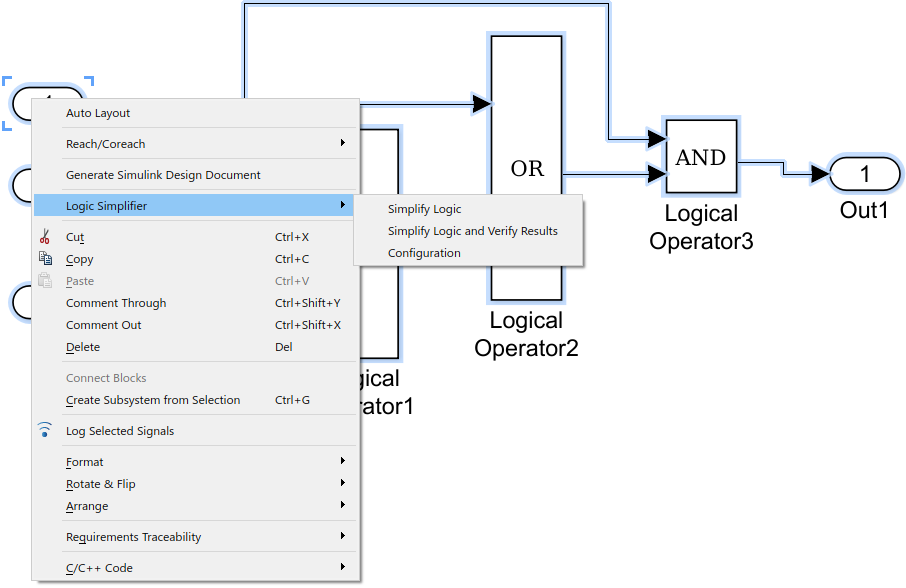
\includegraphics[width=\textwidth]{../figs/ContextMenu}
	\caption{\Simulink Context Menu with tool options visible.}
	\label{FIG:contextMenu}
\end{figure}

%---------------------------------------
% What are the main uses of the tool?
%---------------------------------------
\subsection{Functionality}
\label{SEC:functionality}
This section describes the tool functionality when it is used from the \Simulink Context Menu (Figure~\ref{FIG:contextMenu}).

\subsubsection*{\menu{1}}
Right-clicking on a selection of blocks in a system, and then selecting \cmd{\menu{1}} from the Context Menu will:
\begin{enumerate} \label{enum:menu1}
  \item Create a ``new logic model'' with the filename being the system containing the selected blocks with \file{\_newLogic.slx} appended along with a number to make the filename unique if needed\footnote[1]{\label{fn:sys-invalid-model-name}When this tool creates a model, it is always saved in the \keyword{Logic\_Simplifier\_Results} folder which is found with the rest of the files for the tool. 
  When this tool names a model, if the name is not a valid model name, instead of using the name of the original system in the filename, \keyword{DefaultModel} is used.}.
  \item Simplify the selection of blocks and generate it in the new logic model along with the remaining blocks from the system containing the selected blocks\footnote[2]{\label{fn:assume-default}Assumes default configuration parameters.}.
  Users should analyze the simplification to make sure that it is correct.
  \item The Auto Layout Tool will be run on the simplified blocks.
  Other blocks will be mostly undisturbed from the original system except from being shifted to avoid overlapping with the new blocks.
\end{enumerate}

\subsubsection*{\menu{2}}
Right-clicking on a selection of blocks in a system, and then selecting \cmd{\menu{2}} from the Context Menu will:
\begin{enumerate} \label{enum:menu2}
  \item Perform all of the steps performed by the \nameref{enum:menu1} option.
  \item Create a ``harnessed model'' with the filename being the system containing the selected blocks with \file{\_orig\_with\_harness.slx} appended along with a number to make the filename unique if needed\footref{fn:sys-invalid-model-name}.
  %\item Copy the selected blocks into the ``harnessed model'' preserving signal lines connecting them.
  %Goto/From/DataStoreWrite/DataStoreRead blocks that lead outside of the system and unconnected ports are fed to inport and outport blocks (this is the ``harness'').
  \item Create a ``harnessed new logic model'' with the filename being the system containing the selected blocks with \file{\_newLogic\_with\_harness.slx} appended along with a number to make the filename unique if needed\footref{fn:sys-invalid-model-name}.
  %\item Copy the simplified blocks of the ``new logic model'' into the ``harnessed new logic model'' preserving signal lines connecting them.
  %Goto/From/DataStoreWrite/DataStoreRead blocks that lead outside of the system and unconnected ports are fed to inport and outport blocks (this is the ``harness''). 
  %\textit{Note: The harness is still a work in progress. 
  %In a correct harness, the inport and outport numbers between the ``harnessed model'' and the ``harnessed new logic model'' should correspond with the same logic of the model.}
  \item Create a ``verification model'' with the filename being the system containing the selected blocks with \file{\_verify.slx} appended along with a number to make the filename unique if needed
%  \footref{fn:sys-invalid-model-name}.
  \footnote[1]{\label{fn:sys-invalid-model-name}When this tool creates a model, it is always saved in the \keyword{Logic\_Simplifier\_Results} folder which is found with the rest of the files for the tool. 
  When this tool names a model, if the name is not a valid model name, instead of using the name of the original system in the filename, \keyword{DefaultModel} is used.}.
  \item The ``verification model'' will feed the same inputs to the harnessed models and compare values of the outputs via the \verb|==| operator and send the results to Design Verifier Proof Objectives.
  The user should select \cmd{Analysis > Design Verifier > Prove Properties > Model} from the menubar.
  If in the results summary shows that all objectives were processed and proven valid and that 0 were falsified, then the simplification was valid (shown in Figure~\ref{FIG:demo4}).
  Otherwise the simplification produced an incorrect result or the verification model was not generated properly (or both).
\end{enumerate}

\subsubsection*{\menu{3}}
Right-clicking anywhere in the model and then selecting \cmd{Logic Simplifier > \menu{3}} from the Context Menu, will open the configuration file for the tool (\file{\toolFolder\textbackslash src\textbackslash config.txt}). The following options are available to the user, and can be modified to fit the user's needs.

\begin{itemize}
	\item \cmd{subsystem\_rule} -- Customize handling of subsystems. 
	\item \cmd{blocks\_to\_simplify} -- Customize which blocks to simplify. 
	\item \cmd{generate\_mode} -- Customize which blocks to generate.
	\item \cmd{extra\_support} -- Customize handling of different block/mask types (Advanced).
\end{itemize}

Please see the configuration file for more details regarding parameter usage and accepted values. 
These parameters can be modified with \Matlab open, and do not require that \Matlab be restarted for the changes to take effect.

%---------------------------------------
% What else does the tool do?
%---------------------------------------

\subsection{Errors and Warnings}
Any errors or warnings during tool use will be visible in the \Matlab Command Window. Typically, errors will be shown when the model is locked or function parameters are incorrect.

A common warning occurs when the model's \param{UnderspecifiedInitializationDetection} parameter is not set to \param{Classic}. This parameter must be set to \param{Classic} in order for the tool to provide more reliable simplification results.
The warning follows:
\begin{verbatim}
  Warning: The SimplifyLogic function may result in unexpected 
  results if the `UnderspecifiedInitializationDetection' model 
  parameter is not set to `Classic', please check the results 
  carefully.
\end{verbatim}

\subsection{Known Bugs}
There are a few known bugs that users should be aware of:
\begin{enumerate}
	\item \switch and \ifblk blocks may be over-simplified in cases where they pass non-Boolean values. This is caused due to the tool translating \switch and \ifblk blocks into equivalent representations using \cmd{\&, |, $\sim$, <, <=, >, >=, ==, $\sim$=} (the underlying simplification engine uses this representation).
	
	\item When the verification model is created, two ``harnessed models'' are created along with it.
	One of the models is created by first copying the blocks selected for simplification into a model 
	and then unused input ports, unused output ports, and \block{Goto}s, \block{From}s, \block{Data Store Read}s, and \block{Data Store Write}s that send a signal out of the selected blocks are each connected to an \block{Inport}s or \block{Outport}s.
	The other model does the same with the simplified blocks.
	This functionality is not fully functional as the added \block{Inport}s and \block{Outport}s need to correspond with the same equivalent logic in both models and this will not always be the case.
	This functionality also currently fails when some inputs are unused after simplification because they were redundant originally.
	Therefore, in general, the harness should not fail if it is not needed and all inputs are needed.
	The harness is not needed when there are no unused input ports, unused output ports, and no blocks sending implicit data outside the selection.
\end{enumerate}

%%%%%%%%%%%%%%%%%%%%%%%%%%%%%%%%%%%%%%%%%%%%%%%%%%%%%%%%%%%%%%%%%%%
% Example
%%%%%%%%%%%%%%%%%%%%%%%%%%%%%%%%%%%%%%%%%%%%%%%%%%%%%%%%%%%%%%%%%%%
\section{Example}
Use the command \demoName in the \Simulink command window to open the example model, shown in Figure~\ref{FIG:demo1}.

\begin{figure}[!htb]
  \centering
	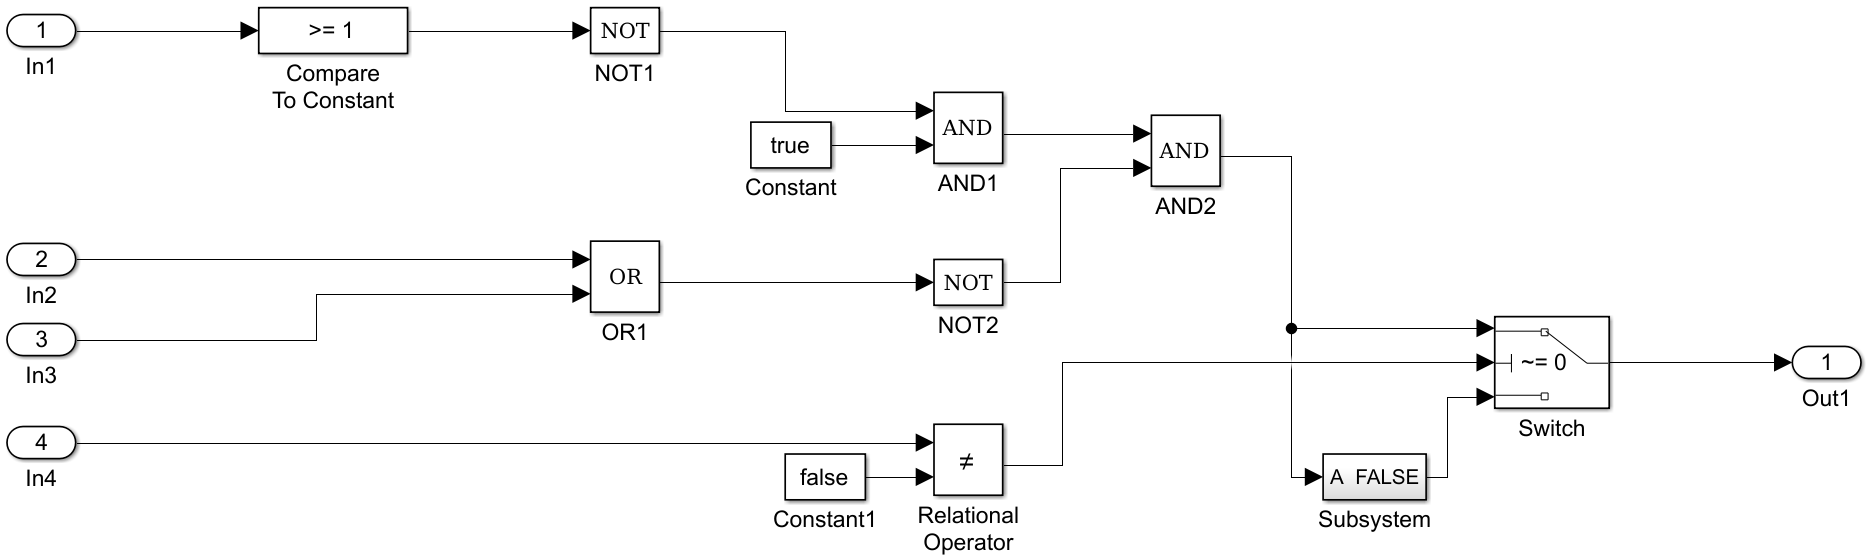
\includegraphics[width=.9\textwidth]{../figs/SimplifierDemo}
	\caption{Demo model before simplification.}
	\label{FIG:demo1}
\end{figure}

To simplify this logic, select all the blocks, \eg with \cmd{ctrl+A}. Then, right-click any of the blocks and select \cmd{Logic Simplifier > \menu{1}} from the Context Menu. 
The resulting model opens automatically and is shown in Figure~\ref{FIG:demo2}\footref{fn:sys-invalid-model-name}. 
We can see many simplifications have occurred:
\begin{itemize}
  \item \block{NOT1} was removed, and the operator parameter in \block{Compare To Constant} was simplified to the less than (\textless) operator, as shown in \block{gen\_RelationalOp} of the simplified model. This is a valid simplification because if A is not greater than or equal to 1, then one can equivalently say that A is less than 1 ($\neg (A >= 1) \Leftrightarrow	 (A < 1)$).
  \item DeMorgan's Law ($\neg(A\lor B) \Leftrightarrow (\neg A\land \neg B)$) was applied over \block{OR1} and \block{NOT2}. This produced a logical \AND operation with \NOT{s} on its inputs. %($\sim$(A\cmd{|}B) = ($\sim$(A)\&$\sim$(B)))
  \item A \block{true} constant fed into \block{AND1}. Using the Identity Law ($A\land1 \Leftrightarrow	 A$), this can be simplified to remove the \block{true} input of the \AND.
  \item In the original model, a \block{false} constant and \block{In4} fed into a $\neq$ \relational. This was simplified to simply use \block{In4}. Note that this simplification in and of itself is invalid if \block{In4} does not output a Boolean.
  \item The \block{Subsystem} contained logic which reduced to false. This reduction occurred because the \param{subsystem-rule} parameter of the configuration file was set to \param{full-simplify}.
  \item \block{Switch} passed its first input when \block{In4} was true, and otherwise passed its third input which was always false. This simplified to a logical \AND of the first and second inputs.
  \item There were numerous logical \AND{s} with two inputs during the simplification that eventually reduced to a single logical \AND with four inputs.
\end{itemize}
In other words the tool did all these simplifications so the user did not have to.

\begin{figure}[!htb]
  \centering
	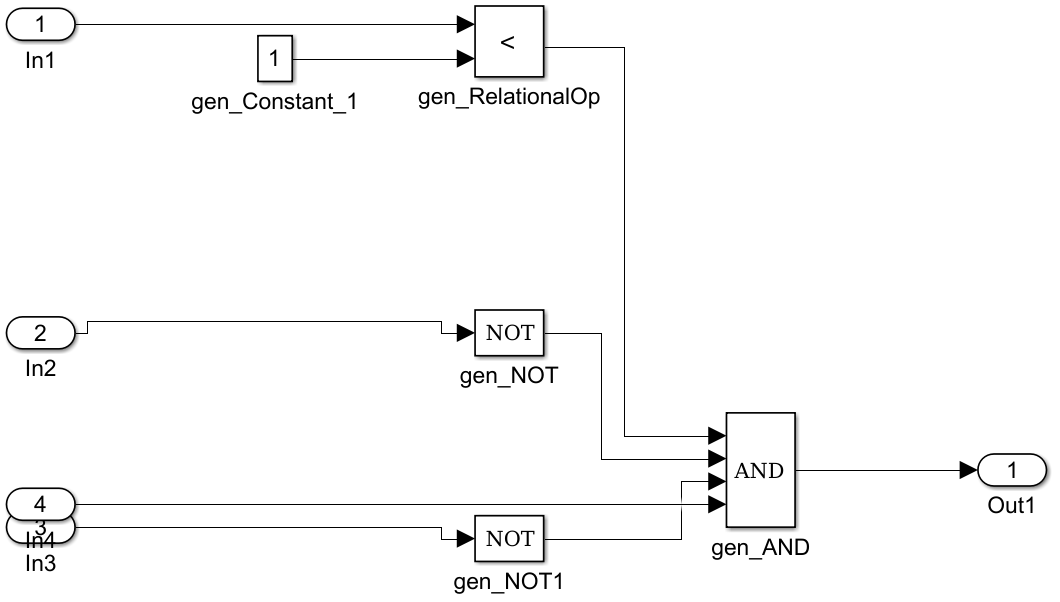
\includegraphics[width=.9\textwidth]{../figs/SimplifierDemo-Simplified}
	\caption{Demo model after simplification.}
	\label{FIG:demo2}
\end{figure}

To perform the same simplification, but also prove that the simplified model is behaviourally equivalent to the original, select the \cmd{\menu{2}} option instead. This will create the simplified model shown in Figure~\ref{FIG:demo2}, but also create a verification model, shown in Figure~\ref{FIG:demo3}.

\begin{figure}[!htb]
  \centering
	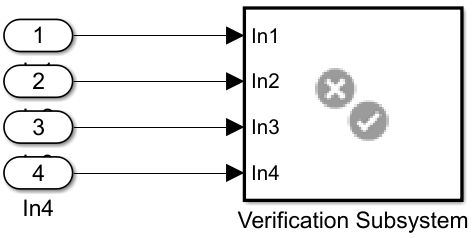
\includegraphics[width=.7\textwidth]{../figs/VerificationModel}
	\caption{Generated verification model.}
	\label{FIG:demo3}
\end{figure}

To begin the property proving, select \cmd{Analysis > Design Verifier > Prove Properties > Model} from the menubar, as shown in Figure~\ref{FIG:ProveStart}.

\begin{figure}[!htb]
  \centering
	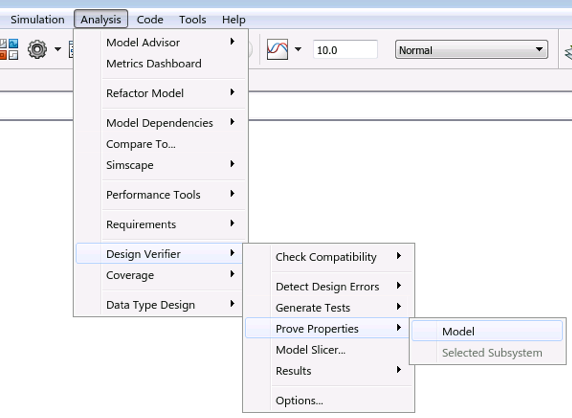
\includegraphics[width=.9\textwidth]{../figs/StartProve}
	\caption{How to begin property proving.}
	\label{FIG:ProveStart}
\end{figure}

A ``\SDV Results Summary" window will open and display the progress of this operation, as shown in Figure~\ref{FIG:demo4}. Once the proving operation is complete, the summary window will update to show how many of the properties it was able to prove to be valid or false. The number of properties corresponds to the number of outputs that should be equivalent. Detailed result reports are available in the links.

\begin{figure}[!htb]
  \centering
	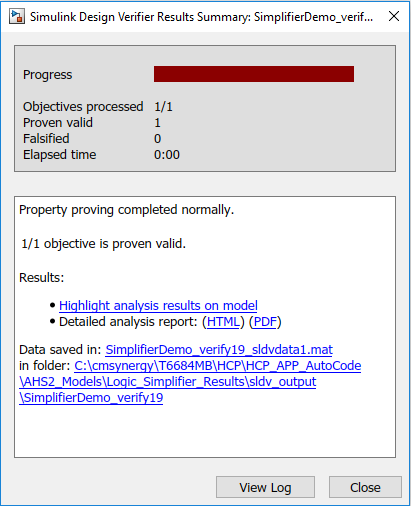
\includegraphics[width=0.8\textwidth]{../figs/VerificationResults}
	\caption{\SDV results summary, with all objectives processed and proven valid.}
	\label{FIG:demo4}
\end{figure}

%%%%%%%%%%%%%%%%%%%%%%%%%%%%%%%%%%%%%%%%%%%%%%%%%%%%%%%%%%%%%%%%%%%
% Matlab Commands
%%%%%%%%%%%%%%%%%%%%%%%%%%%%%%%%%%%%%%%%%%%%%%%%%%%%%%%%%%%%%%%%%%%
\clearpage
\section{Matlab Commands}

The tool can also be used via the \Matlab command line, with the following functions.

%---------------------------------------
% Command 1
%---------------------------------------
\begin{center}
	\begin{tabular}{| >{\columncolor[gray]{0.9}}l | p{10.5cm} |} \hline
		Function 			& \cmd{\func{1}} \\ \hline
		Syntax				& \cmd{[newEqu, oldEqu] = \func{1}}(\args{blocks}, \args{varargin}) \\ \hline
		Description		& Construct a model with simplifications of the given blocks (\ie perform the same steps as the \nameref{enum:menu1} option from the GUI). \\ \hline
		Inputs				& \args{blocks}: Cell array of blocks (indicated by fullname). \\[.5em] 
              		& \args{varargin}: Boolean indicating whether or not to verify the results. Defaults to false. [Optional] \\ \hline
		Outputs				& \args{newEqu}: Cell array of equations found for the blocks as given. \\[.5em]
              		& \args{oldEqu}: Cell array of equations found for the blocks after the simplification process. \\ \hline
	\end{tabular}
\end{center}

%---------------------------------------
% Command 2
%---------------------------------------
\begin{center}
	\begin{tabular}{| >{\columncolor[gray]{0.9}}l | p{10.5cm} |} \hline
		Function 			& \cmd{\func{2}} \\ \hline
		Syntax				& \cmd{verificationModel = \func{2}}(\args{address}, \args{model1}, \args{model2}, \args{saveDir}) \\ \hline
		Description		& Construct a model (\file{.mdl}) which can be used to verify equivalence between two models using \SDV. \\ \hline
		Inputs			& \args{address}: Verification model name. \\[.5em]
								& \args{model1}: First model to verify. \\[.5em]
								& \args{model2}: Second model to verify.\\[.5em]
								& \args{saveDir}: Fullpath of directory to save the constructed model in.\\ \hline
		Outputs			& \args{verificationModel}: Fullpath of location and name of the constructed model.\\ \hline	
	\end{tabular}
\end{center}

%---------------------------------------
% Command 3
%---------------------------------------

%\begin{center}
%	\begin{tabular}{| >{\columncolor[gray]{0.9}}l | p{10.5cm} |} \hline
%		Function 		& \\ \hline
%		Syntax			& \\ \hline
%		Description		& \\ \hline
%		Inputs			& \\ \hline	
%		Outputs 		& \\ \hline	
%	\end{tabular}
%\end{center}

\end{document}